\chapter{Анализ предметной области}

В данном разделе будут введены основные определения и будет обоснована актуальность задачи внесения изменений в ядро операционной системы Linux.

\section{Актуальность}

Программное обеспечение с открытым исходным кодом имеет такие преимущества, как скорость разработки и надежность. Причиной этого является большое число участников разработки. Каждый разработчик находит ошибки, представляет их решение и предлагает новый функционал. Так, осуществляется непрерывный процесс внесения изменений.

Ядро Linux --- программное обеспечение с открытым исходным кодом, поэтому непрерывно разрабатывается специалистами со всего мира. Добавление новых функций, внесение усовершенствований, исправление ошибок делают актуальной проблему внесения изменений в ядро операционной системы Linux.

\section{Основные определения}

Ядро операционной системы --- это программное обеспечение, которое предоставляет базовые функции для всех остальных частей операционной системы, управляет аппаратным обеспечением и распределяет системные ресурсы \cite{love}.

Одной из характеристик ядра Linux является динамическая загрузка модулей ядра. Другими словами, при необходимости существует возможность динамической загрузки и выгрузки исполняемого кода во время работы системы. Так, можно переопределять или дополнять функции ядра. Файлы с исправлениями встраиваются в виде загружаемых модулей ядра.

Технику внесения изменений в код или данные, позволяющую модифицировать поведение целевого алгоритма требуемым образом, называют патчингом \cite{patching}. Патчи --- это небольшие добавочные изменения, вносимые в ядро. Каждый патч содержит изменение ядра, реализующее одну независимую модификацию.

При примении патча к ядру операционной системы необходимо знать состояние функций ядра, используется ли функция в момент исправления или нет. Для этого используется метод обхода стека.

\begin{figure}[H]
	\begin{center}
		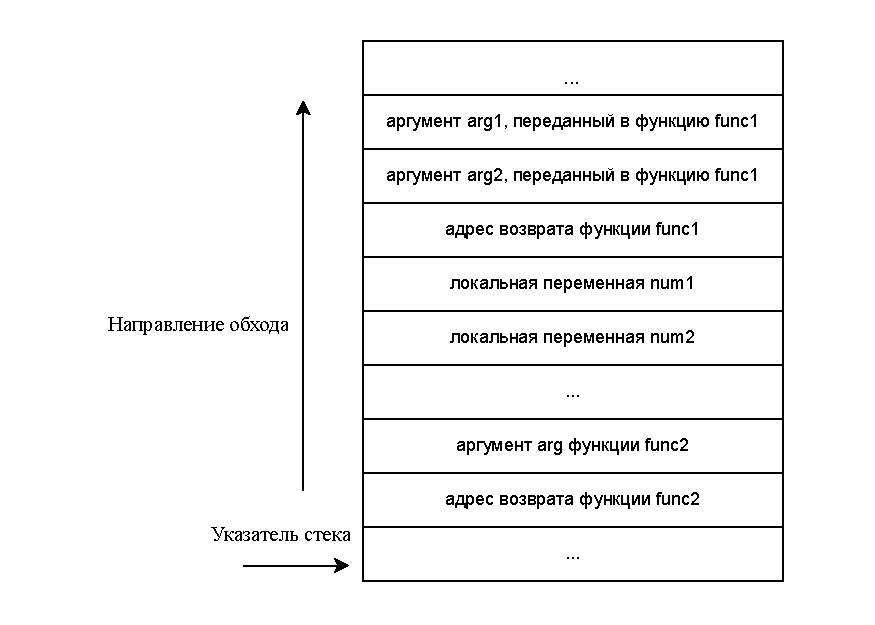
\includegraphics[scale=0.9]{img/call-stack.pdf}
	\end{center}
	\captionsetup{justification=centering}
	\caption{Метод обхода стека}
	\label{img:call-stack}
\end{figure}

В методе обхода стека проверяется стек вызовов каждого потока ядра, показанный на рисунке \ref{img:call-stack}. Необходимо определить, выполняется ли поток в функции, которую необходимо изменить. Для этого копия указателя стека уменьшается пока значение не достигнет нижней части стека. Функция используется, если адрес, принадлежащий этой функции можно найти в стеке.


\section{Вывод}

Были изучены основные определения и была обоснована важность проблемы изменения ядра операционной системы Linux.